\documentclass[aps,pre,amsmath,amssymb,floatfix,onecolumn,notitlepage,10pt]{revtex4-1}
\usepackage{graphicx,isomath}
\usepackage[colorlinks=true,linkcolor=blue,citecolor=blue,urlcolor=blue,pdfborderstyle={/S/U/W 1}]{hyperref}

\begin{document}

\title{Continuation of Janus chimeras}
\author{Zachary G. Nicolaou}
\date{\today}

\maketitle
%%%%%%%%%%%%%%%%%%%%%%%%%%%

\section{Introduction}
Complex patterns of synchronization can emerge in networks of coupled oscillators.  Recently, for example, a myriad of localized traveling chimera states were reported to occur in a remarkably simple model known as the ring of Janus oscillators \cite{2019_Nicolaou}. Localized oscillatory states have also been noted in heterogeneous arrays of parameterically-driven pendula \cite{2021_Nicolaou_1}, which have been of interest in the study of classical time crystals \cite{2021_Nicolaou_2}.  In other contexts, localized steady solutions are known to occur through universal snaking bifurcations. The snaking bifurcations of steady solutions in the one-dimensional Swift-Hohenberg equation, for example, can be understood through the winding geometry of homoclinic and heteroclinic orbits \cite{2006_burke, 2009_beck}. In higher spatial dimensions, snaking bifurcations of steady solutions are known to exhibit  more complex features, such as multiple snaking branches and isolas \cite{2019_bramburger,2020_bramburger}. The study of snaking bifurcations has previously focused on steady-state solutions to ordinary and partial differential equations, but patterns of synchrony typically exhibit nonstationary dynamics.  There is a potential for the geometric interpretation of steady state snaking bifurcations to extend to snaking of limit cycle or chaotic attractors. However, since limit cycles can exhibit both period doubling and torus bifurcations in additional to fold bifurcations, they have the potential to exhibit novel snaking phenomena not possible for steady state solutions, which only exhibit fold and Hopf bifurcaitons.  The purpose of these notes is to investigate whether the emergence of localized patterns of synchrony can be related to previous understanding of steady state snaking bifurcations.

\section{Janus oscillators}
\subsection{Complex equations}
We aim to study the bifurcations in the ring of Janus oscillators, defined by the equations
\begin{align}
\dot{\theta}_n &= \omega/2 + \beta\sin(\phi_n - \theta_n) + \sigma \sin(\phi_{n+1}-\theta_n), \label{janus1}\\
\dot{\phi}_n &= -\omega/2 + \beta\sin(\theta_n - \phi_n) + \sigma \sin(\theta_{n-1}-\phi_n), \label{janus2}
\end{align}
with $n=N+m$ identified with $n=m$ for periodic boundary conditions. These equations are known to support localized and attractive traveling chimera solutions, and we ask whether these solutions emerge from universal a snaking bifurcation process.
For the sake of numerical continuation, we consider the complex equations
\begin{align}
\dot z_n &= z_n\left( i\omega/2 + \beta/2\left(w_nz_n^*-z_nw_n^*\right) + \sigma/2\left(w_{n+1}z_n^*-z_nw_{n+1}^*\right)\right) + \gamma\left(1-z_nz_n^*\right)z_n, \label{eom1} \\
\dot w_n &= w_n\left( -i\omega/2 + \beta/2\left(z_nw_n^*-w_nz_n^*\right) + \sigma/2\left(z_{n-1}w_n^*-w_nz_{n-1}^*\right)\right) + \gamma\left(1-w_nw_n^*\right)w_n. \label{eom2}
\end{align}
Denote the polar coordinates as $z_n = \rho_n{\mathrm e}^{i\theta_n}$ and $w_n = \eta_n{\mathrm e}^{i\phi_n}$ and the Cartesian coordinates as $z_n = x_n + iy_n$ and $w_n = u_n+iv_n$. Straightforward change of variables leads to the polar equations of motion
\begin{align}
\dot \rho_n &= \gamma \rho_n \left(1-\rho_n^2\right), \\
\dot \eta_n &=  \gamma \eta_n \left(1-\eta_n^2\right),  \\
\dot \theta_n &= \omega/2 + \beta \rho_n \eta_n \sin\left(\phi_n-\theta_n\right) + \sigma \rho_n\eta_{n+1}\sin\left(\phi_{n+1}-\theta_n\right)\\
\dot \phi_n &= -\omega/2 + \beta \rho_n \eta_n \sin\left(\theta_n-\phi_n\right) + \sigma \rho_{n-1} \eta_n\sin\left(\theta_{n-1}-\phi_n\right).
\end{align}
Note that the amplitude dynamics decouples from the phases and are attracted to the fixed points $\rho_n=1$ and $\eta_n=1$.  Thus, we can initialize the equations with unit amplitudes, and the amplitude dynamics become irrelevant.  The phase equations reduce to the ring of Janus oscillators in Eqs.~\eqref{janus1}-\eqref{janus2}. The major advantages of the complex representation for numerical continuation is that, unlike the phases, the variables remain bounded in time and the limit-cycle attractors are periodic in the complex variables.  To integrate these bounded variables numerically, we express the evolution in Cartesian coordindates,
\begin{align}
\dot x_n &= -y_n\left(\omega/2 - \beta \left(-x_nv_n+u_ny_n \right) - \sigma\left(-x_nv_{n+1}+u_{n+1}y_n\right) \right) + \gamma\left(1-x_n^2-y_n^2\right)x_n, \\
\dot y_n &= x_n\left(\omega/2 - \beta \left(-x_nv_n+u_ny_n \right) - \sigma\left(-x_nv_{n+1}+u_{n+1}y_n\right) \right) + \gamma\left(1-x_n^2-y_n^2\right)y_n, \\
\dot u_n &= -v_n\left(-\omega/2 - \beta \left(-u_ny_n+x_nv_n \right) - \sigma\left(-u_ny_{n-1}+x_{n-1}v_n\right) \right) + \gamma\left(1-u_n^2-v_n^2\right)u_n, \\
\dot v_n &= u_n\left(-\omega/2 - \beta \left(-u_ny_n+x_nv_n \right) - \sigma\left(-u_ny_{n-1}+x_{n-1}v_n\right) \right) + \gamma\left(1-u_n^2-v_n^2\right)v_n.
\end{align}

\subsection{Time-shift reductions for chimera states}
The chimera state solutions in the ring of Janus oscillators are traveling waves. We cannot change to moving spatial coordinates since the lattice is discrete, but we can instead consider the time-delayed coordinate $\tau_n = t - \nu n$ for oscillator $n$, where $1/\nu$ is the velocity. We can enact a reduction if we assume that the oscillator dynamics are identical in their respective time-delayed coordinates (i.e., the variables depend on time only through the invariant coordinate $\tau_n$). Additionally, the space translational invariance and the invariance under global phase rotations enables a reduction, which we call the cluster-twisted traveling wave ansatz: $z_n(t) = e^{i\eta n}\left(X_{n\,\text{mod}\,q}(t-\nu n)+iY_{n\,\text{mod}\,q}(t-\nu n)\right)$ and $w_n(t) = e^{i\eta n}\left(U_{n\,\text{mod}\,q}(t-\nu n)+iV_{n\,\text{mod}\,q}(t-\nu n)\right)$, where $q$ denotes the number of clusters and $\eta$ is twist parameter, and $\nu$ is, again, the velocity.  Inserting this ansatz into Eqs.~\eqref{eom1}-\eqref{eom2}, taking $X_m + iY_m = e^{i\Theta_m}$, $U_m+iV_m=e^{i\Phi_m}$, and ignoring the (transient) amplitude dynamics, we find a set of $2q$ time-shift equations
\begin{align}
\dot{\Theta}_m(\tau) &= \omega/2 + \beta\sin(\Phi_m(\tau)-\Theta_m(\tau)) + \sigma\sin(\Phi_{m+1\, \text{mod}\, q}(\tau-\nu) -\Theta_m(\tau)-\eta), \label{timeshift1} \\
\dot{\Phi}_m(\tau) &= -\omega/2 + \beta\sin(\Theta_m(\tau)-\Phi_m(\tau)) + \sigma\sin(\Theta_{m-1\, \text{mod}\, q}(\tau+\nu) -\Phi_m(\tau)+\eta). \label{timeshift2}
\end{align}
Given a chimera state from numerical simulations, we can attempt to fit $\eta$, $\nu$, and $q$ in order to reduce the solution to a limit-cycle solution of Eqs.~\eqref{timeshift1}-\eqref{timeshift2} with period $T$. On a ring of $N$ Janus oscillators, periodicity in space implies that $N\nu = p T$ for some integer $p$, so that $\nu = pT/N$. In the limit of large $N$, the chimera solutions correspond to a localized disturbance in $\Theta_m(\tau)$ and $\Phi_m(\tau)$, with asymptotic $\tau \to \pm \infty$ behavior corresponding to a steady state of $q$-clustered synchrony with twisting rate determined by $\eta$. In principle, these localized solutions may undergo snaking bifurcations, leading to chimera states with groups of co-traveling asynchronous regions. The time delay here complicates this analysis somewhat both theoretically and numerically, however.

\subsection{Discrete symmetries in the ring}
The ring of Janus oscillators is not reflection symmetric for $\sigma \neq \beta$, since the coupling between $\theta$ and $\phi$ variables has an inherent chirality. Instead, Eqs.~\eqref{janus1}-\eqref{janus2} posses at least two discrete parity-reversing symmetries. First, the ring is invariant under the time/parity reversal $\pi_1$ given by $(\theta_n',\phi_n',t') = \pi_1(\theta_n,\phi_n,t) \equiv (\pi+\phi_{N-n},\theta_{N-n},-t)$. (By invariant, we mean that under the change of coordinates from $(\theta_n,\phi_n,t)$ to $(\theta_n',\phi_n',t')$, the new governing are identical to the original equations.)
Since this map reverses the direction of time, stable solutions are mapped to unstable solutions under $\pi_1$.  Second, the ring is invariant under the parity/sign reversal $(\theta_n',\phi_n',t') = \pi_2(\theta_n,\phi_n,t) \equiv (-\phi_{N-n},-\theta_{N-n},t)$. Since the direction of time is preseved by this map, the map $\pi_2$ takes stable solutions to other stable solutions.  Note that the parity/sign reversal symmetry leaves the Kuramoto order parameter invariant as well (so there are two branches of solutions corresponding to each line in the bifurcation diagrams below). Composition of the two parity symmetries gives a time/sign reversal symmetry $\pi_3$ defined by $(\theta_n',\phi_n',t')=\pi_3(\theta_n,\phi_n,t)\equiv(\pi-\theta_n,-\phi_n,-t)$. Lastly, the ring is invariant under discrete rotations defined by $(\theta_n',\phi_n',t')=R(\theta_n,\phi_n,t)\equiv(\theta_{n+1},\phi_{n+1},t)$, taking the periodic boundary conditions into account.

\subsection{Accommodating continuous symmetries in AUTO}
Since the phase equations depend only on phase differences, the equations are invariant under global phase rotations $\theta_i\to\theta_i+\psi$ and $\phi_i\to \phi_i+\psi$.  This means that limit cycle attractors and fixed point attractors will have a neutrally stable perturbation direction corresponding to phase rotations. For limit cycle attractors, with the additional neutral perturbation corresponding to time shifts $\theta_i\to\theta_i+\epsilon\dot{\theta_i}$ and $\phi_i\to\phi_i+\epsilon\dot{\phi_i}$, there will be two unit Floquet multipliers for all parameter values, rendering all points singular in the pseudo-arclength continuation method employed by AUTO. To fix this problem, we could change variables to include the conserved quantity $\Theta = \sum_n \left(\theta_n + \phi_n\right)$ in the Janus ring. In such coordinates, the conserved quantities will decouple from a reduced system, and we can study stability in the reduced system instead.  A slightly simpler reduction in the ring of Janus oscillators can be made by moving into a reference frame that rotates at the speed of, say, oscillator $z_0$. Define quantities $\tilde{z}_n = z_n/z_0$ and $\tilde{w}_n = w_n/z_0$ (whose phases are, respectively, $\theta_n-\theta_0$ and $\phi_n-\theta_0$).  Then $\dot {\tilde z}_n = \dot z_n / z_0 - \left(z_n/z_0\right)\left( \dot z_0/z_0\right)$ and $\dot {\tilde w}_n = \dot w_n / z_0 - \left(w_n/z_0\right) \left(\dot z_0/z_0\right)$. Assuming (wlog) that $z_0$ is initialized with $z_0=1$, we then have upon substituting into Eqs.~\ref{eom1}-\ref{eom2}
\begin{align}
\dot {\tilde z}_n &= i{\tilde z}_n\left(  \beta/2\left({\tilde w}_n{\tilde z}_n^*-{\tilde z}_n{\tilde w}_n^* - {\tilde w}_0+{\tilde w}_0^*\right) + \sigma/2\left({\tilde w}_{n+1}{\tilde z}_n^*-{\tilde z}_n{\tilde w}_{n+1}^* - {\tilde w}_1+{\tilde w}_1^*\right)\right) + \gamma\left(1-{\tilde z}_n{\tilde z}_n^*\right){\tilde z}_n, \label{janus_rot1}\\
\dot {\tilde w}_n &= i{\tilde w}_n\left( -\omega + \beta/2\left({\tilde z}_n{\tilde w}_n^*-{\tilde w}_n{\tilde z}_n^* -{\tilde w}_0^*+{\tilde w}_0 \right) + \sigma/2\left({\tilde z}_{n-1}{\tilde w}_n^*-{\tilde w}_n{\tilde z}_{n-1}^* - {\tilde w}_1+{\tilde w}_1^*\right)\right) + \gamma\left(1-{\tilde w}_n{\tilde w}_n^*\right){\tilde w}_n. \label{janus_rot2}
\end{align}
It is straightforward to continue of the Cartesian form of Eqs.~\eqref{janus_rot1}-\eqref{janus_rot2} in AUTO.

\subsection{Numerical continuation}
We have continued chimera branches in a ring of $16$ Janus oscillators using custom python code and AUTO. Figure \ref{fig1} shows the results of this continuation. OBSERVATIONS: i) The period of each chimera branch increases with the continuation and eventually causes a stop. Is this a sign that they undergo SNIC? Can we find the corresponding saddle and node? ii) Chimera branches have a dual time/parity reversal. Several branches appear become self-dual at a limit point around $0.25<\sigma<0.27$. This is a branch point, since all Floquet multipliers must be neutrally stable by symmetry. AUTO struggles here, and our python BVP may be improved. Can we implement the OK Floquet multipliers in solvebvp??

NOTE: We should continue the unstable steady cluster twisted solutions! They will probably appear in the SNICs, and the chimeras can be understood as a continuation of the heteroclinic connection.

\begin{figure}[hb]
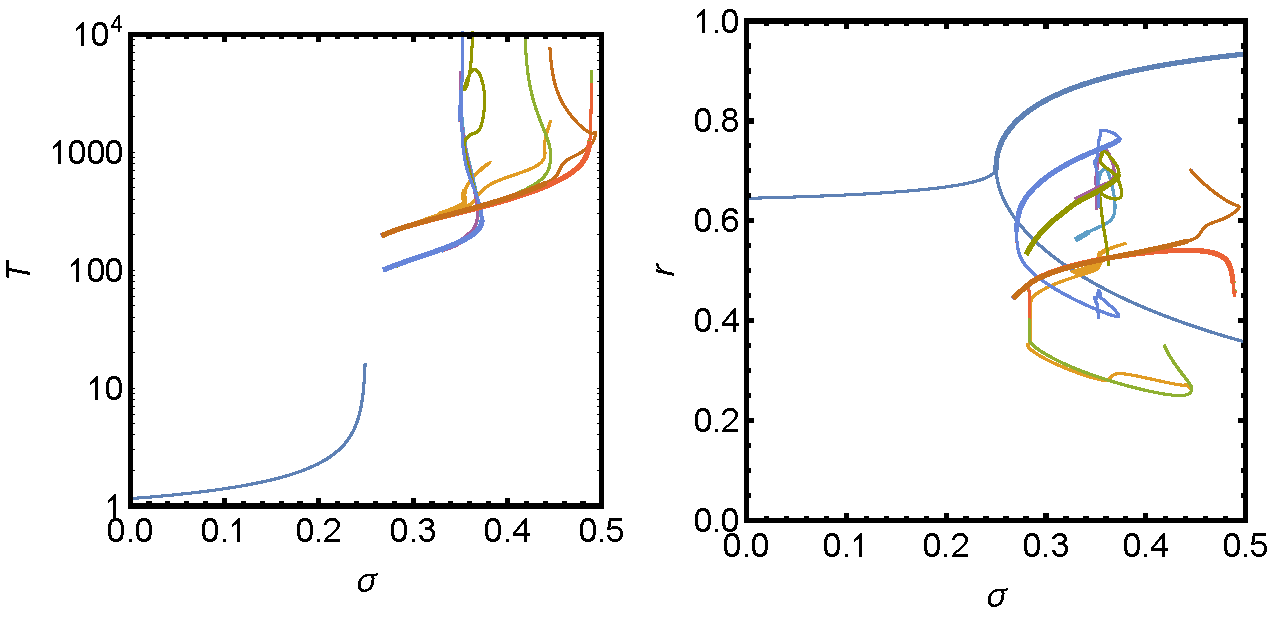
\includegraphics[width=\columnwidth]{diagram.pdf}
\caption{Bifurcation diagram with the synchronous stable branch (thick red), synchronous unstable branch (thin black), stable limit-cycle chimeras (green dots), and unstable limit-cycle chimeras (blue circles). \label{fig1}}
\end{figure}


\section{Parametrically-driven pendula}
\subsection{Complex equations}
We now consider the parametrically-driven array of pendula with alternating lengths, as described in \cite{2021_Nicolaou_1,2021_Nicolaou_2}.  Let $\theta_n$ and $\phi_n$ be the angles the $n$th long and short pendula make with the vertical direction, respectively. As for the ring of Janus oscillators, we again employ a complex representation $z_n=e^{i\theta_n}$ and $w_n=e^{i\phi_n}$. Since the model is second order in time, we introduce the auxiliary momenta variables $p_n = \dot{\theta}_n$ and $q_n=\dot{\phi}_n$.  Lastly, we introduce a auxiliary complex variable $Z$ evolving according to the Stuart-Landau equation, which acts as the periodic drive on the pendula. The complex equations of motion can be written as
\begin{align}
\dot{z}_n&=iz_np_n/(1+\Delta)+\gamma(1-|z_n|^2)z_n \\
M\dot{p}_n&=-\eta p_n+(Mg+a_d\omega_d^2\frac{Z+Z^*}{2}-4\kappa\Delta)\frac{z_n-z_n^*}{2i} +\kappa(1-\Delta)\frac{(w_n+w_{n+1})z_n^*-(w_n^*+w_{n+1})z_n}{2i} \\
\dot{w}_n&=iw_nq_n/(1-\Delta)+\gamma(1-|w_n|^2)w_n \\
M\dot{p}_n&=-\eta q_n+(Mg+a_d\omega_d^2\frac{Z+Z^*}{2}+4\kappa\Delta)\frac{w_n-w_n^*}{2i} +\kappa(1+\Delta)\frac{(z_n+z_{n-1})w_n^*-(z_n^*+z_{n-1})w_n}{2i}\\
\dot{Z}&=IZ+\gamma(1-|Z|^2)Z.
\end{align}

\subsection{Discrete symmetries}
The pendulum array is reflection symmetric and has a translational symmetry. This allows the wavemode decomposition of the perturbation of the homogeneous state, but note that the $q$ and $-q$ modes have degenerate Floquet modes. Since the $q=\pm\pi$ modes are identical, the period doubling solution can be continued without degnerate Floquet modes, but this is not so for the $|q|<\pi$ modes. They do not mix because of the translation symmetry, but this means that pairs of modes exhibit the period doubling bifurcations at exactly the same driving.  Thus, the branch of solutions remains degenerate in the Floquet multipliers. Can we defined a user stopping condition to detect special BP points that have higher degeneracy?

\begin{thebibliography}{99}
\bibitem{2019_Nicolaou} Z. G. Nicolaou, D. Eroglu, and A. E. Motter. Multifaceted dynamics of Janus oscillator networks. \textit{Phys. Rev. X} \textbf{9}, 011017 (2019).
\bibitem{2021_Nicolaou_1} Z. G. Nicolaou, D. J. Case, E. B. Van der Wee, M. M. Driscoll, and A. E. Motter. Heterogeneity-stabilized homogeneous states in driven media. \textit{Nature communications} \textbf{12}, 4486 (2021).
\bibitem{2021_Nicolaou_2} Z. G. Nicolaou and A. E. Motter. Anharmonic classical time crystals: A coresonance pattern formation mechanism. \textit{Physical Review Research} \textbf{3}, 023106 (2021).
\bibitem{2006_burke} J. Burke and E. Knobloch. Localized states in the generalized Swift-Hohenberg equation. \textit{Phys. Rev. E} \textbf{73}, 056211 (2006).
\bibitem{2009_beck} M. Beck, J. Knobloch, D. J. B Lloyd, B. Sandstede, and T. Wagenknecht. Snakes, ladders, and isolas of localized patterns. \textit{SIAM Journal on Mathematical Analysis} \textbf{41}, 936-972 (2009).
\bibitem{2019_bramburger}J. J. Bramburger, D. Altschuler, C. I. Avery, T. Sangsawang, M. Beck, P. Carter, and B. Sandstede. Localized radial roll patterns in higher space dimensions. \textit{SIAM Journal on Applied Dynamical Systems} \textbf{18}, 1420-1453 (2019).
\bibitem{2020_bramburger}J. J. Bramburger, and B. Sandstede. Spatially localized structures in lattice dynamical systems. \textit{Journal of Nonlinear Science} \textbf{30}, 603-644 (2020).
\end{thebibliography}
\end{document}
